
%%%%%%%% HZZ4l %%%%%%%
%%%>  Introduction <%%%

\section{Introduction}
\label{sec:introduction}

The standard model (SM) of electroweak
interactions~\cite{StandardModel67_1,StandardModel67_2,StandardModel67_3}
relies on the existence of the Higgs boson ($\PH$), a scalar particle
of mass $\mH$ associated with the field responsible for the
spontaneous electroweak symmetry
breaking~\cite{Englert:1964et,Higgs:1964ia,Higgs:1964pj,Guralnik:1964eu,Higgs:1966ev,Kibble:1967sv}.
The value of $\mH$ is not fixed by the theory.
%The wealth of electroweak precision
%data from the LEP and SLC colliders, the Tevatron and other experiments
%$predicted the Higgs to be at about 90~\GeV with an upper limit of $152~\GeV$ at
%the 95\% confidence level (CL). 
Direct searches at LEP excluded values lower
than $114.4~\GeV$ at 95\% confidence level (CL)~\cite{Barate:2003sz} and early Tevatron measurements
excluded the mass range $162-166~\GeV$ at 95\% CL~\cite{TEVHIGGS_2010}.
%The discovery or exclusion of the SM Higgs boson is one of the primary scientific goals of 
%the Large Hadron Collider  
%(LHC)~\cite{Evans:2008zzb}.
Previous direct searches at the Large Hadron Collider (LHC)~\cite{Evans:2008zzb} 
were based on data from 
proton-proton (pp) collisions corresponding to 
an integrated luminosity of 5\fbinv collected at a center-of-mass
energy $\sqrt{s}=7$\TeV.
The CMS experiment excluded 
at 95\% CL a range of masses from 127 to 600\,GeV~\cite{Chatrchyan:2012tx}.
The ATLAS experiment excluded at 95\% CL the ranges 111.4--116.4,
119.4--122.1 and 129.2--541\unit{GeV}~\cite{ATLAS:2012ae, atlas:20127tev}.
%Within the remaining allowed mass region, 
An excess of events near 
125\GeV was reported by both experiments. 
In 2012 the $\Pp\Pp$ center-of-mass energy was increased to 8\TeV and by the end of June
an additional integrated luminosity of more than 5\fbinv had been
recorded by each of these experiments, 
thereby enhancing significantly the sensitivity of the search for the Higgs boson.
In an effort to improve the results, the analyses went through a major
optimization process that was also applied to the data taken in 2011. 
The result is the observation of a new heavy boson with a mass of about $125 \,\GeV$ 
%Both LHC experiments, CMS and
%ATLAS, simultaneously published the observation in a concise
%paper
~\cite{CMSobservation125,ATLASobservation125}. 

Given the fact that an overall excess is found at the low end of the 
mass spectrum explored by
both the LHC and Tevatron experiments, the main interest in the Higgs 
searches is currently
focused on that mass region.
Moreover there are classic upper bounds on the Higgs-boson mass coming 
from 
unitarity~\cite{Veltman:1976rt,Lee:1977yc,Lee:1977eg,Passarino:1990hk}, 
triviality and
vacuum stability, precision electroweak data and absence of fine-tuning (for a
recent review see Ref.~\cite{Ellis:2009tp}).
Nevertheless, in view of the role of the Higgs boson in the unitarization of 
the diboson-scattering at high energy,
it is of primary importance to keep studying the high mass region,
in particular processes which involve the vector-boson fusion (VBF) 
production mechanism.

It has been proposed that the low mass boson can be interpreted as 
imposter~\cite{Low:2011gn,Low:2012rj}
with no connection with the electroweak symmetry breaking mechanism. In this
interpretation, the SM Higgs boson has still to be searched for. On the 
other hand, 
%given the compelling role of the
%Higgs in the unitarization of the theory, 
many BSM models, which predict 
the presence of additional resonances
at high mass (Higgs mass splitting), can be built as
modification of the SM case. In all these models, theoretical issues 
related with the width of the resonance
and the interference with the background, will have to be addressed. A 
correct treatment of these
problems needs to be established first in the SM case.
%, as will be shown 
%in the following.

In this paper a search is reported 
using the standard model Higgs boson 
in $\PH \to
\WW$ and $\PH \to \ZZ$ decay channels
as benchmarks for cross section and production mechanism 
%The boson-mass hypotheses are examined 
 in the range $145 < \mH < 1000$ GeV.  
%Because of these reasons, we interpret the results of the analyses in 
%terms of upper
%limits on the cross-section for a SM scenario. 
Despite of the previously 
mentioned theoretical constraints,
this approach is sufficiently well-defined and self-consistent to allow
efficient and coherent presentation of unbiased results. A more general, 
model-independent,
search for beyond-SM heavy resonances is left for future work.

%Given the fact that an overall excess is found at the low end of the
%mass spectrum explored by both the LHC 
%and Tevatron experiments, the
%main interest in the Higgs searches is currently focused on that mass
%region.  It is nevertheless important to keep studying the high mass
%region, in particular processes which involve the vector-boson fusion
%(VBF) production
%mechanism and which are expected to be greatly affected by the
%presence or absense of a Higgs boson-like particle.

For $\mH \ge 2\mW$, the main discovery channels at 
the LHC are those
with two real weak bosons: $\WW$ for $2\mW \le \mH < 2 \mZ$, and
additionally $\ZZ$ for $\mH \ge 2\mZ$.
%There are classic constraints on the Higgs-boson mass coming from
%unitarity~\cite{Veltman:1976rt,Lee:1977yc,Lee:1977eg,Passarino:1990hk}, 
%triviality and
%vacuum stability, precision electroweak data and absence of fine-tuning (for a
%recent review see Ref.~\cite{Ellis:2009tp}).
%In the following we interpret the results of the analyses
%, performed up to very high
%values of the mass, 
%in terms of upper limits on the cross-section for a SM scenario.
%While this approach has obvious problems with the (external) 
%theoretical constraints, it is
%sufficiently well-defined and self-consistent to allow efficient and coherent presentation
%of unbiased results. 
%A more general, model-independent, search for beyond-SM heavy resonances 
%(compatible with the
%125~\GeV discovery~\cite{discovery}) 
%is left for future work.
For a
Higgs boson decaying to two $\PW$ bosons, the fully leptonic ($\PH \to
\WW \to \ell\nu\ell\nu$) and semileptonic ($\PH \to \WW \to \ell \nu
\mathrm{qq}$) final states are considered.  For a Higgs boson decaying into two $\cPZ$
bosons, the final states are studied containing 
four leptons ($\PH \to \ZZ
\to 2\ell 2\ell '$),
two leptons and two
jets ($\PH \to \ZZ \to
2\ell \mathrm{q\bar{q}}$), and two leptons and two neutrinos, ($\PH
\to \ZZ \to 2\ell 2\nu$), 
where $\ell = \Pe$ or $\Pgm$ and $\ell ' = \Pe$ or
$\Pgm$, or $\Pgt$.  The analyses use pp collision data recorded by the
CMS detector, corresponding to integrated luminosities of
5.1 ${\rm fb}^{-1}$ at $\sqrt{s} = 7\TeV$ and 5.3 ${\rm fb}^{-1}$ at
$\sqrt{s} = 8\TeV$.


\section{CMS detector and simulations}
\label{sec:cms}

The central feature of the CMS apparatus~\cite{Chatrchyan:2008zzk} is
a superconducting solenoid of 6\unit{m} internal diameter, which
provides a magnetic field of 3.8\unit{T}. Within the field volume are
a silicon pixel and strip tracker, a lead tungstate crystal
electromagnetic calorimeter (ECAL), and a brass/scintillator hadron
calorimeter (HCAL). 
A quartz-fiber
Cherenkov calorimeter extends the coverage to $|\eta| <$ 5.0, where pseudorapidity
is defined as $\eta=-{\rm ln}[\tan{(\theta/2)}]$,
and $\theta$ is the polar angle of the trajectory of the particle
with respect to the beam direction. 
Muons are measured in gas-ionization detectors
embedded in the steel flux-return yoke. Extensive forward calorimeters
complement the coverage provided by the barrel and endcap detectors.
The first level of the CMS trigger system, composed of custom
hardware processors, is designed to select the most interesting events
in less than 3 $\mu$s using information from the calorimeters and muon
detectors. The High Level Trigger processor farm 
decreases the event rate from 100 kHz delivered by the first level trigger
 to a few hundred Hz, before data storage.

CMS uses a right-handed coordinate system, with the
origin at the nominal interaction point, the $x$ axis
pointing to the center of the LHC ring, the $y$ axis pointing
up (perpendicular to the plane of the LHC ring), and the $z$ axis
along the counterclockwise-beam direction. The polar angle
$\theta$ is measured from the positive $z$ axis and the
azimuthal angle $\phi$ is measured in the $x$-$y$ plane.
The transverse
momentum $\PT = \sqrt{p_x^2 + p_y^2}$.
Missing transverse energy $\met$ is defined as the modulus of the negative vector sum of the
transverse momenta of all reconstructed particles, charged or neutral, in the event.

A number of Monte Carlo (MC) event generators are used to simulate the signals and
backgrounds. 
The $\PH \rightarrow \WW(\ZZ)$
signal 
generated by using the
next-to-leading order (NLO) program {\sc powheg}~\cite{POWHEG}.
The Higgs boson signals from gluon fusion ($\Pg\Pg \rightarrow \PH$),
and vector-boson fusion ($\Pq\Pq \rightarrow \Pq\Pq \PH$), are generated with
{\sc powheg} at NLO and a dedicated
generator from Ref.~\cite{Gao:2010qx} for angular correlations.
Additional samples of \PW\PH, \cPZ\PH, and $\ttbar\PH$ events are generated with
\PYTHIA 6.424~\cite{Sjostrand:2006za}.

Events at generator level are reweighted according to the total cross section $\sigma(\Pp\Pp\rightarrow \PH)$,
which contains contributions from gluon fusion up to next-to-next-to-leading order (NNLO) and next-to-next-to-leading log taken from
Refs.~\cite{Anastasiou:2008tj,deFlorian:2009hc,Baglio:2010ae,LHCHiggsCrossSectionWorkingGroup:2011ti,Djouadi:1991tka,Dawson:1990zj,Spira:1995rr,Harlander:2002wh,Anastasiou:2002yz,Ravindran:2003um,Catani:2003zt,Actis:2008ug}
and from the  weak-boson fusion contribution computed at NNLO in
Refs.~\cite{LHCHiggsCrossSectionWorkingGroup:2011ti,Ciccolini:2007jr,Ciccolini:2007ec,Figy:2003nv,Arnold:2008rz,Bolzoni:2010xr}.
%The total cross section is scaled by the branching fractions calculated
%with \textsc{prophecy4f}, which includes NLO QCD and electroweak corrections and
%all interference effects at NLO~\cite{LHCHiggsCrossSectionWorkingGroup:2011ti,Bredenstein:2006rh,Bredenstein:2006ha,hdecay2,Actis:2008ts}, in particular effects specific to the $4\Pe$ and $4\Pgm$
%channels.

%There are classic constraints on the Higgs boson mass coming from
%unitarity~\cite{Veltman:1976rt,Lee:1977yc,Lee:1977eg,Passarino:1990hk}, 
%triviality and
%vacuum stability, precision electroweak data and absence of fine-tuning (for a
%recent review see Ref.~\cite{Ellis:2009tp}).
%In the following we interpret the results of the analyses, performed up to very high
%values of the mass, in terms of upper limits on the cross-section for a SM scenario.
%While this approach has obvious problems with the (external) 
%theoretical constraints, it is
%sufficiently well-defined and self-consistent to allow efficient and coherent presentation
%of unbiased results. 
%A more general, model-independent, search for beyond-SM heavy resonances (compatible with the
%125~\GeV discovery~\cite{discovery}) is left for future work.

\begin{figure}[htbp]
\centering
   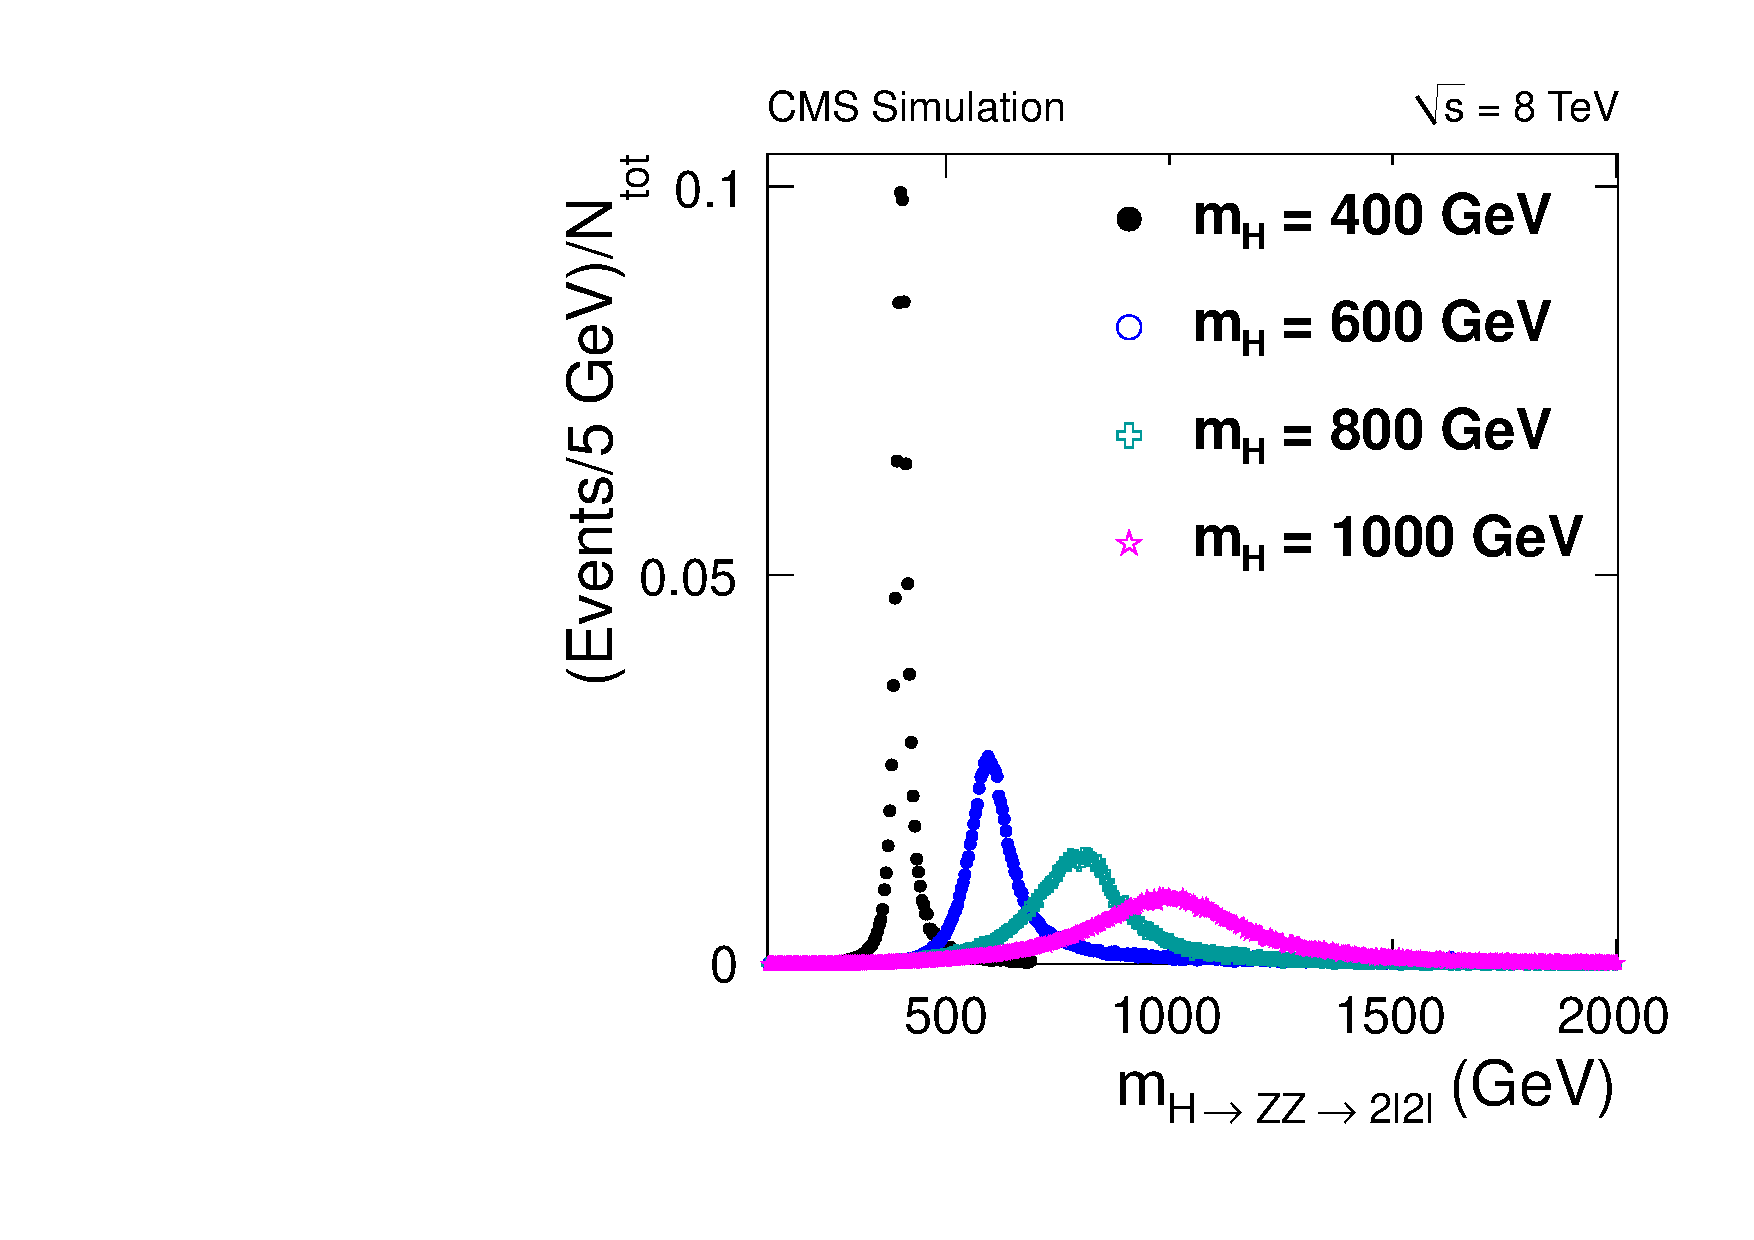
\includegraphics[width=0.6\textwidth]{figures/HiggsMasses.pdf}
   \caption{Distributions of the Higgs boson mass for different $m_{\rm{H}}$
    hypotheses obtained from simulated events, after corrections explained in the text.
    The area of each distribution is normalized to unity.
   }
\label{fig:higgsmasses}
\end{figure}

The \WW(\ZZ) invariant mass ($m_{\WW(\ZZ)}$) lineshape is corrected to match the results
presented in Ref.~\cite{Passarino:2010qk,Goria:2011wa,Kauer:2012hd},
where the complex-mass scheme (CPS) for the Higgs propagator is used.
The resulting mass shapes obtained using simulated events
 for different $\mH$ hypotheses are shown in Fig.~\ref{fig:higgsmasses}.
In the gluon-gluon fusion production channel the effects on the
lineshape due to the interference between Higgs-boson signal and the 
$\mathrm{gg} \to \WW(\ZZ)$
background is included, as suggested in Ref.~\cite{Passarino:2012ri}.
The theoretical uncertainty on the lineshape 
%of the resonance 
due to missing higher-order corrections
in the interference between background and signal are included, 
as well as the uncertainties due to electroweak
corrections, as suggested in Refs.~\cite{Goria:2011wa,Passarino:2012ri}.
The contribution of the interference away from the Higgs mass 
%peak of the resonance has
has sizable effects on the normalization for those final states where the 
invariant mass
cannot be fully reconstructed. This correction is included, with the corresponding
theoretical uncertainties, 
in the $\WW \to \ell \nu \rm{qq}$ final state, as suggested in Ref.~\cite{Passarino:2012ri}.
In the $\WW \to \ell\nu\ell\nu$ and $\ZZ \to \ell \ell \nu\nu$ final states, 
the effect of interference on 
the normalization,
as computed in ~\cite{Campbell:2011cu,Kauer:2012ma,MaltoniInPrep},
is included with 100\% uncertainty.
%The effect of interference
%in the VBF production is still under study.




The background contribution from $\rm{q\bar{q}} \to \WW$ production is generated
with the \MADGRAPH~\cite{Alwall:2007st},
% event generator.
the subdominant $\mathrm{gg} \to \WW$ process
%, which is expected to 
%contribute 3\% of the total $\WW$ production rate~\cite{MCFM}, 
is generated 
%by using 
with {\tt gg2ww}~\cite{ggww}.
The $\rm{q\bar{q}} \to \ZZ$ production is generated at 
NLO with 
\POWHEG,
the $gg \rightarrow \ZZ $ 
%signal component 
is estimated 
%using events
%generated using 
with {\tt gg2ZZ} ~\cite{Binoth:2008pr}.
Other diboson processes ($\PW\cPZ$, $\cPZ\gamma$, $\PW\gamma^{(*)}$) are generated with \PYTHIA and 
\MADGRAPH.
%The $\cPZ b\bar{b}$, $\cPZ c\bar{c}$, and Z+light jets, 
The $\cPZ$+jet samples 
are generated with \MADGRAPH. The $\ttbar$ and $\tw$ events are generated at NLO with 
\POWHEG.
For leading-order (LO) generators, the default 
set of parton distribution functions
(PDF) used to produce these samples is \textsc{cteq6l}~\cite{CTEQ66}, while
\textsc{CT10}~\cite{ct10} is used for NLO generators.
The $\Pgt$-lepton decays are generated with \textsc{TAUOLA}~\cite{Jadach:1993hs}.
For all processes, the detector response is simulated using a detailed
description of the CMS detector, based on the \GEANTfour~
package~\cite{GEANT}, and event reconstruction is performed with
the same algorithms as used for data.
The simulated samples are reweighted according to the distribution of number of pp interactions
per bunch crossing (pileup) as measured in the data.

\section{Event reconstruction}
\label{sec:reconstruction}

A complete reconstruction of the individual particles emerging from
each collision event is obtained via a particle-flow (PF) technique.
This uses the information from all CMS sub-detectors to identify and
reconstruct individual particles in the collision
event~\cite{CMS-PAS-PFT-09-001, CMS-PAS-PFT-10-002}, with particles
classified into mutually exclusive categories: charged hadrons,
neutral hadrons, photons, electrons, and muons.
%
%\subsection{Electrons}

The electron reconstruction combines the information from clusters of energy
deposits in the ECAL and the trajectory in the inner
tracker~\cite{Baffioni:2006cd,CMS-PAS-EGM-10-004}.  
%The track-cluster
%matching is initiated either "outside-in" from energy cluster
%measurements, or "inside-out" from track reconstruction.  
Trajectories
in the tracker volume are reconstructed using a dedicated modeling of
the electron energy loss and fitted with a Gaussian sum filter.
%Electrons are identified among the reconstruction candidates and then
%used, together with the other PF particles, to obtain a consistent
%description of the event.  Their identification relies on a
The electron identification relies on a
multivariate technique that combines observables sensitive to the
amount of bremsstrahlung along the electron trajectory, the
geometrical and momentum matching between the electron trajectory and
associated clusters, as well as shower-shape observables.

%
%\subsection{Muons}
The muon reconstruction combines the information from both the silicon
tracker and the muon spectrometer.  
%The matching between the inner and
%outer tracks is initiated either "outside-in", starting from a track
%in the muon system, or "inside-out", starting from a track in the
%silicon tracker.  
The PF muons are selected among the reconstructed
muon-track candidates by applying minimal requirements on the track
components in the muon system and taking into account a matching with
energy deposits in the calorimeters~\cite{CMS-PAS-PFT-10-003}.

%\subsection{Taus}
Tau leptons are identified in their leptonic decay mode 
%denoted
%$\taul$, 
with an electron or muon as measurable decay product, and in
the hadronic one denoted $\tauh$, with hadrons in the decay products.
The PF particles are used to reconstruct $\tauh$ with the
``hadron-plus-strip'' (HPS) algorithm~\cite{Chatrchyan:2011xq}.  The
HPS algorithm optimizes the reconstruction and identification of
specific $\tauh$ decay modes.  
%The $\pi^0$ components of the $\tauh$
%are first reconstructed and then combined with charged hadrons to
%reconstruct the $\tauh$ decay modes.  The neutrinos produced in all
%$\Pgt$ decays escape detection and are ignored in the reconstruction.

%\subsection{Jets}
Jets are reconstructed from PF candidates by using the
anti-$\mathrm{k_{T}}$ clustering algorithm
\cite{Cacciari:2008gp,fastjetmanual} with a distance parameter 
$R = 0.5$. 
Jet-energy corrections are applied to account for the non-linear
response of the calorimeters to the particle energies and other
instrumental effects.  These corrections are based on in-situ
measurements using dijet and $\gamma+{\rm jet}$ data
samples~\cite{Chatrchyan:2011ds}.  
%Pile-up and the underlying event
%have an effect on jet reconstruction by contributing additional energy
%to the reconstructed jets.  
The median energy density due to pileup
is evaluated in each event and the corresponding energy is subtracted
from each jet~\cite{Cacciari:2008gn}.  
%A jet requirement, primarily
%based on the energy balance between charged and neutral hadrons in a
%jet, is applied to remove misidentified jets.
The jets are checked for consistency 
of their origin with the primary vertex based on their impact parameter
significance~\cite{CMS-PAS-BTV-11-003}, where
the
primary vertex is chosen as the vertex with the highest sum of $\PT^2$
of its constituent tracks. 
Based on this check the jets displaced for the primary 
vertex can be tagged as $b$-jets.

%\subsection{b-tagging}
%We use a $b$-tagging veto to reject the top-quark background.
%Top-quark decays are characterized by the presence of jets originating
%from \cPqb\ quarks (\cPqb jets), which can be tagged by using the
%likelihood that the tracks associated to a 
%The jets are checked for consistency to
%come from the primary vertex based on their impact parameter
%significance~\cite{CMS-PAS-BTV-11-003}.  
%The $b$-jets are tagged, since they 
%contain tracks from decays of long-lived particles such as
%$B$ hadrons and therefore are displaced form the primary vertex.  
%The top-quark background is suppressed by applying a
%veto on events having a \cPqb\ tagged jet with transverse energy
%greater than 30\GeV that lies within the tracker volume ($|\eta| <
%2.5$).

%\subsection{Isolation}
%\label{sec:iso}
The isolation of individual $\Pe$ or $\Pgm$ leptons is measured relative
to their 
%transverse momentum 
$\PT^{\ell}$, by summing over charged and
neutral particles in a cone $\Delta R = \sqrt{(\eta^\ell - \eta^i)^{2}
+ (\phi^\ell- \phi^i)^{2}} < 0.4$ around the lepton direction at the
interaction vertex:
\begin{equation*}
R_{\rm Iso}^{\ell} \equiv \left( \sum  \PT^{\rm charged} + {\rm MAX}\left[ 0, \sum \ET^{\rm neutral} 
            +  \sum {\ET}^{\gamma} - \rho \times A_{\rm eff},  \right] \right) /  \PT^{\ell} ~~ .
\end{equation*}
The $\sum \PT^{\rm charged}$ is the scalar sum of the transverse
momenta of charged hadrons originating from the primary vertex.  
%The
%primary vertex is chosen as the vertex with the highest sum of $\PT^2$
%of its constituent tracks.  
The $\sum \ET^{\rm neutral}$ and $\sum
{\ET}^{\gamma}$ are the scalar sums of the transverse energies for
neutral hadrons and photons, respectively.  
%The latter excludes
%photons that are candidates for final-state radiation (FSR) from the
%lepton (see below).  
The term $\rho \times A_{\rm eff}$ subtracts an
estimate obtained using a "jet area" technique~\cite{Cacciari:2007fd}
of the transverse energy from neutrals in the isolation cone coming
from pileup of additional pp collisions.  The transverse energy
density $\rho$ is calculated in each event as the median of the
neutral-energy distribution around "jets" (any PF jet in the event
having $\PT^{\rm jet} > 3$ GeV) with mean effective $\eta-\phi$ area
$A_{\rm eff}$.  
%A small residual dependence on the number of pileup
%collisions is absorbed as a correction factor on $A_{\rm eff}$.

The efficiencies for the trigger requirements and product of reconstruction, identification,
and isolation of primary $\Pe$ or $\Pgm$ leptons are measured in data,
using a tag-and-probe technique~\cite{CMS:2011aa} based on an
inclusive sample of \cPZ\ events.  The measurements are performed in
several bins of $\PT^{\ell} $ and $ |\eta^{\ell}| $.  The efficiencies for
selecting electrons in the ECAL barrel (endcaps) varies from about
71\% (65\%) for $7 < \PT^{\Pe} < 10\GeV$ to 82\% (73\%) at $\PT^{\Pe}
\simeq 10\GeV$, and reaches 90\% (89\%) for $\PT^{\Pe} \simeq 20\GeV$.
It drops to about 85\% in the transition region, $1.44 < |\eta^{\Pe}| <
1.57$, between the ECAL barrel and endcaps.  The muons are
reconstructed and identified with efficiencies above ${\sim}98\%$ in
the full $|\eta^{\Pgm}| < 2.4$ range.  The performance for the tau
lepton identification is discussed in Ref.~\cite{Chatrchyan:2011xq}.
Its efficiency is about 50\% for $\pt^\Pgt > 20\GeV$.
\section{Search channels}
\label{sec:analyses}

The final results presented in this paper are obtained by combining 
the results from the searches for the Higgs boson
exploiting different production and decay modes. 
A summary of all analyses 
is presented in Table~\ref{tab:channels}, where we list their main characteristics, namely:
exclusive final states,
the mass range of the search (full range is given for each analysis, 
the results at $\mH < 145\GeV$ are presented in ~\cite{CMSobservation125}),
%the integrated luminosity used,
the approximate instrumental mass resolution.
All final states are inclusive, there is no overlap between channels.
The presence of a signal or an upward fluctuation of the background in one of the channels, 
at a certain value of the Higgs boson mass, is expected to manifest itself as an excess 
extending around that value for a range corresponding to the $\mH$ resolution, which 
also includes the effect of reconstruction.
It is important to mention that presence of the boson with $\mH = 125\GeV$ is not
taken into account, and its possible contribution to measurements at higher masses
is not corrected for. This can lead to overestimate in observed signal for
channels with pure mass resolution at low mass region of this analysis, and therefore
to increase in the exclusion limit.

\begin{table}[htbp]
\begin{center}
\small
\caption{Summary information on the analyses included in this paper. All final states are exclusive.
Notations used are: 
$(jj)_{VBF}$ -- dijet pair consistent with the VBF topology;  
$(jj)_{\PW(\cPZ)}$ -- dijet pair with an invariant mass consistent with coming from a 
$\PW(\cPZ)$ dijet decay; 
the column ``\PH prod'' indicates which production mechanism is targeted by an analysis; it does not imply 100\% purity.
The main contribution in the untagged and inclusive categories is always gluon-gluon fusion.    
}
\label{tab:channels}
\begin{tabular}{|l|c|l| ccc|}
\hline
\multicolumn{3}{|c|}{} & No. of & $m_{\PH}$ range  & $m_{\PH}$  \\
\PH decay & \PH prod  & Exclusive final states & channels  & (\GeV)  & resolution \\
\hline\hline
%--------------------------------------------------------------------------------------------------------------------------------------------------------------------------------------------------------------------------------------------------
$\PW\PW \to \ell\nu\ell\nu$      & 0/1-jets  &  ($\Pe\Pe$, $\Pgm\Pgm$, $\Pe\Pgm$) + (0 or 1 jets) &  4         & 110--600         & 20\%  \\ 
$\PW\PW \to \ell\nu\ell\nu$      & VBF-tag    &  $ ($\Pe\Pe$, $\Pgm\Pgm$, $\Pe\Pgm$) + (jj)_{VBF}$  & 1 or 2    & 110--600         & 20\%  \\ 
$\PW\PW \to \ell\nu qq$          & untagged  &  $(\Pe\nu, \, \Pgm\nu) + $($(jj)_{\PW}$ with 0 or 1 jets) & 4    & 170--600         & 5--15\%  \\ 
\hline%--------------------------------------------------------------------------------------------------------------------------------------------------------------------------------------------------------------------------------------------------
$\cPZ\cPZ \to 2\ell 2\ell'$             & inclusive  &  $4\Pe, \, 4\Pgm, \, 2\Pe2\Pgm$                                                                          & 3         & 110--1000         & 1-2\%   \\  
      &   &  $(\Pe\Pe, \, \Pgm\Pgm) + (\Pgt\Pgt)$                        & 8         & 200--1000         & 10-15\%  \\  
$\cPZ\cPZ \to 2\ell 2q$          & inclusive  &  $(\Pe\Pe,\Pgm\Pgm) + $($(jj)_{\cPZ}$ with 0, 1, 2 b-tags)                                           & 6         & 200--600 & 3\% \\ 
$\cPZ\cPZ \to 2\ell 2\nu$        & untagged  &  $(\Pe\Pe,\Pgm\Pgm)$ + MET + 0, 1, 2 non-VBF jets                                        & 6       & 200--1000         & 7\%   \\
$\cPZ\cPZ \to 2\ell 2\nu$        & VBF-tag    &  $(\Pe\Pe,\Pgm\Pgm)$ + MET + $(jj)_{VBF}$                                                           & 2         & 200--1000         & 7\%   \\
\hline%--------------------------------------------------------------------------------------------------------------------------------------------------------------------------------------------------------------------------------------------------
\end{tabular}
\end{center}
\end{table}


The combination of the Higgs boson searches
requires simultaneous analysis of the data selected by all individual analyses,
accounting for all statistical and systematic uncertainties and their correlations.
The overall statistical methodology used in this combination was developed 
by the ATLAS and CMS Collaborations in the context of the LHC Higgs Combination Group.
The description of the general methodology can be found in Refs.~\cite{LHC-HCG-Report, CMScombFeb2012}. 

